% ------------------------------------------------
\StartChapter{LaTex Symbol寫法}{appendix:unicode-symbols}
% ------------------------------------------------

這部份資料來源是xeCJK的v3.3.4(2016/02/10)版本中提供的50頁有關所有Symbol的寫法, 極度值得同學們閱讀或在這邊找你所需的Symbols.\\

內容的說明方式為:\\
Symbol: 符號所顯示的樣子\\
USV: 以Unicode方式所代表的這個符號, 例如 `(' 的Unicode寫法為U+0028.\\
Description: 是這符號的名字.\\
Macro(s): 是LaTex使用這符號的寫法.\\

\textbf{P.S: }因為符號數量多, 沒法100\%保證全能使用.

\setboolean{@twoside}{false}
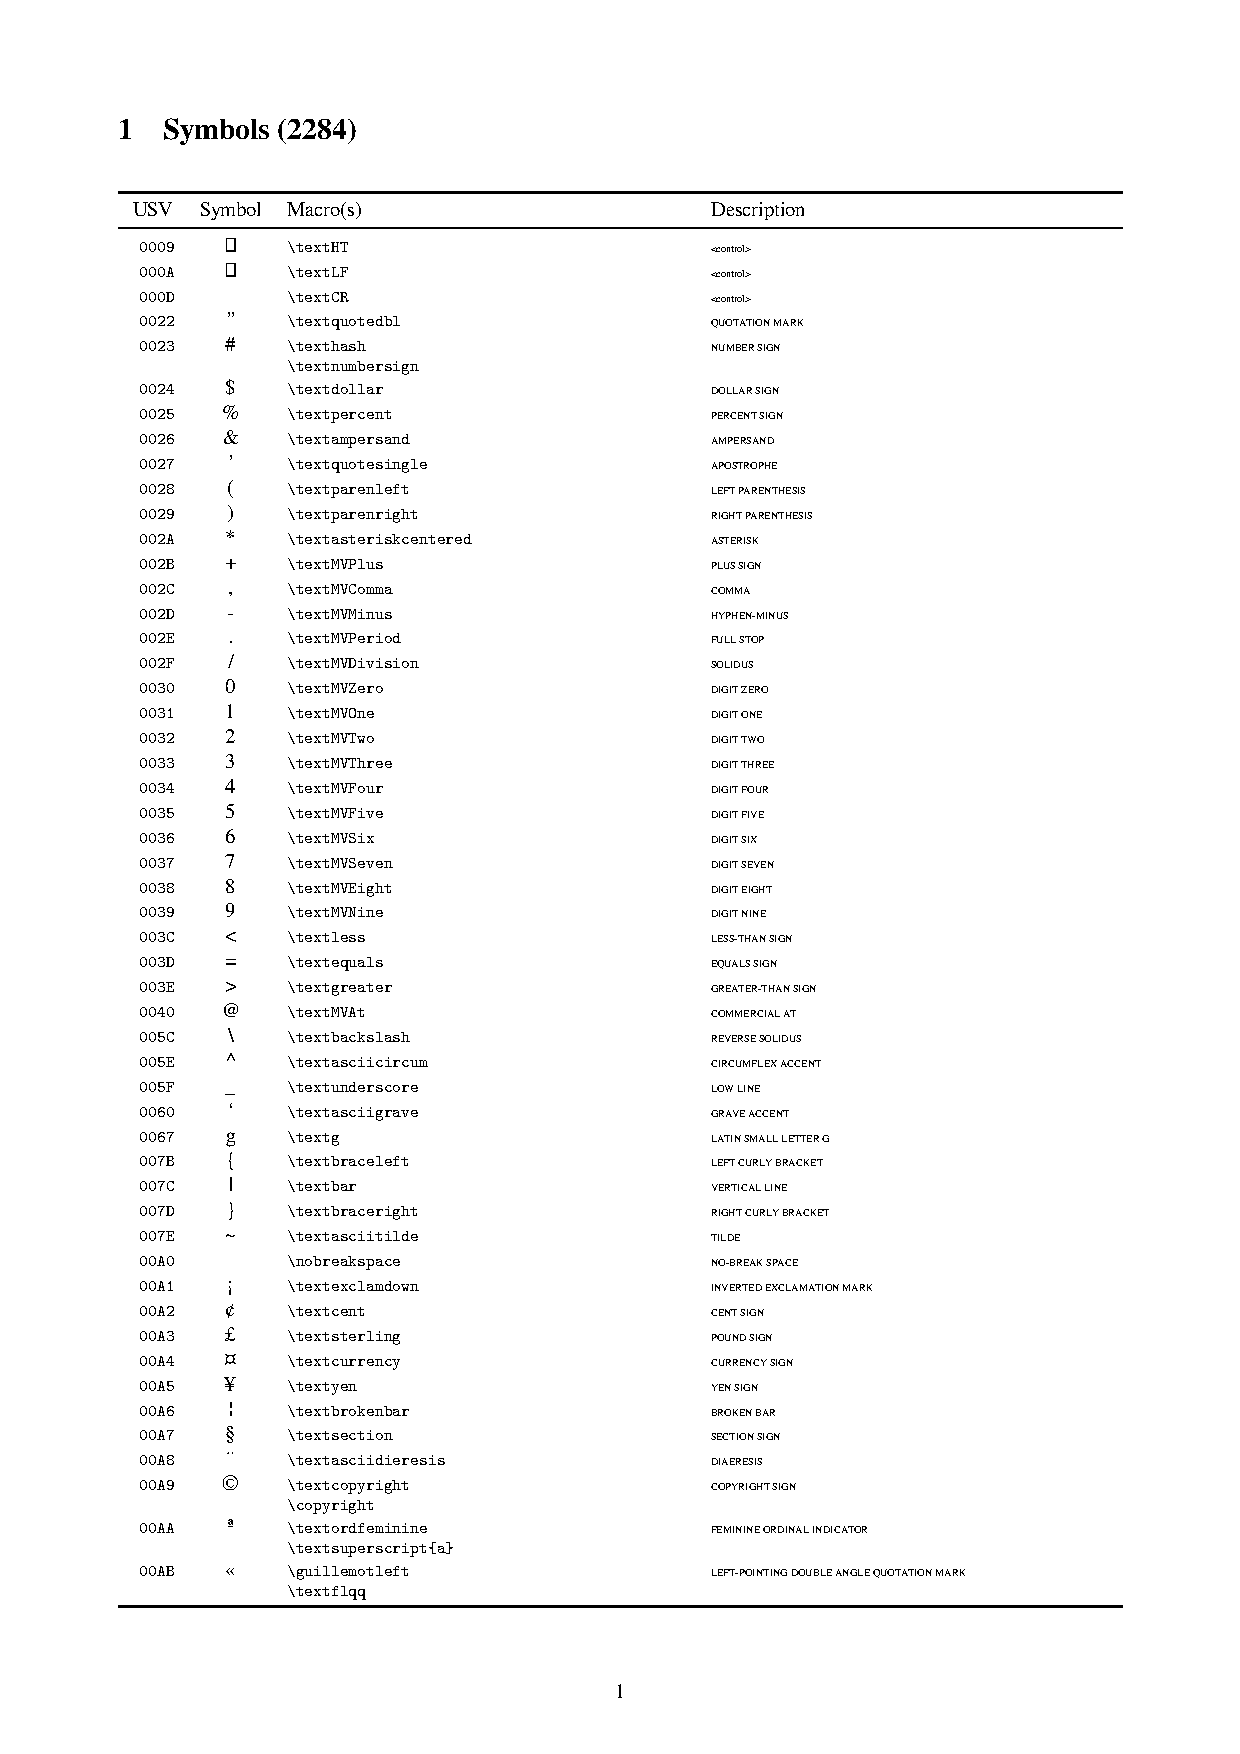
\includepdf[pages=-]{./example/appendix/pdf/xunicode-symbols.pdf}

% ------------------------------------------------
\EndChapter
% ------------------------------------------------
